\documentclass{scrartcl}
\usepackage[mathletters]{ucs}
\usepackage[utf8x]{inputenc}
\usepackage{amssymb}
\usepackage{amsmath}
\usepackage[usenames]{color}
\usepackage{hyperref}
\usepackage{wasysym}
\usepackage{graphicx}
\usepackage[normalem]{ulem}
\usepackage{enumerate}

\usepackage{listings}

\lstset{ %
basicstyle=\footnotesize,       % the size of the fonts that are used for the code
showspaces=false,               % show spaces adding particular underscores
showstringspaces=false,         % underline spaces within strings
showtabs=false,                 % show tabs within strings adding particular underscores
frame=single,                   % adds a frame around the code
tabsize=2,                      % sets default tabsize to 2 spaces
breaklines=true,                % sets automatic line breaking
breakatwhitespace=false,        % sets if automatic breaks should only happen at whitespace
}


\title{Masterproef Tool Wear Inspection - Update 3 DH}
\date{dinsdag 08 december 2020}
\author{}

\begin{document}

\maketitle

		\section{Masterproef Tool Wear Inspection - Update 3 DH}

Created vrijdag 20 november 2020



\subsection{Mail}

Beste meneer Hulens,

 

Ik heb mijn eerste beeldjes kunnen maken met het geautomatiseerd systeem.

Een foto van de opstelling die ik nu gebruik zit in bijlage, hierbij zijn er twee bogen waarop een enkel adresseerbare ledstrip is geplaatst. De ene boog kan nog vrij draaien om de hoek tussen de twee ledstrips aan te passen.



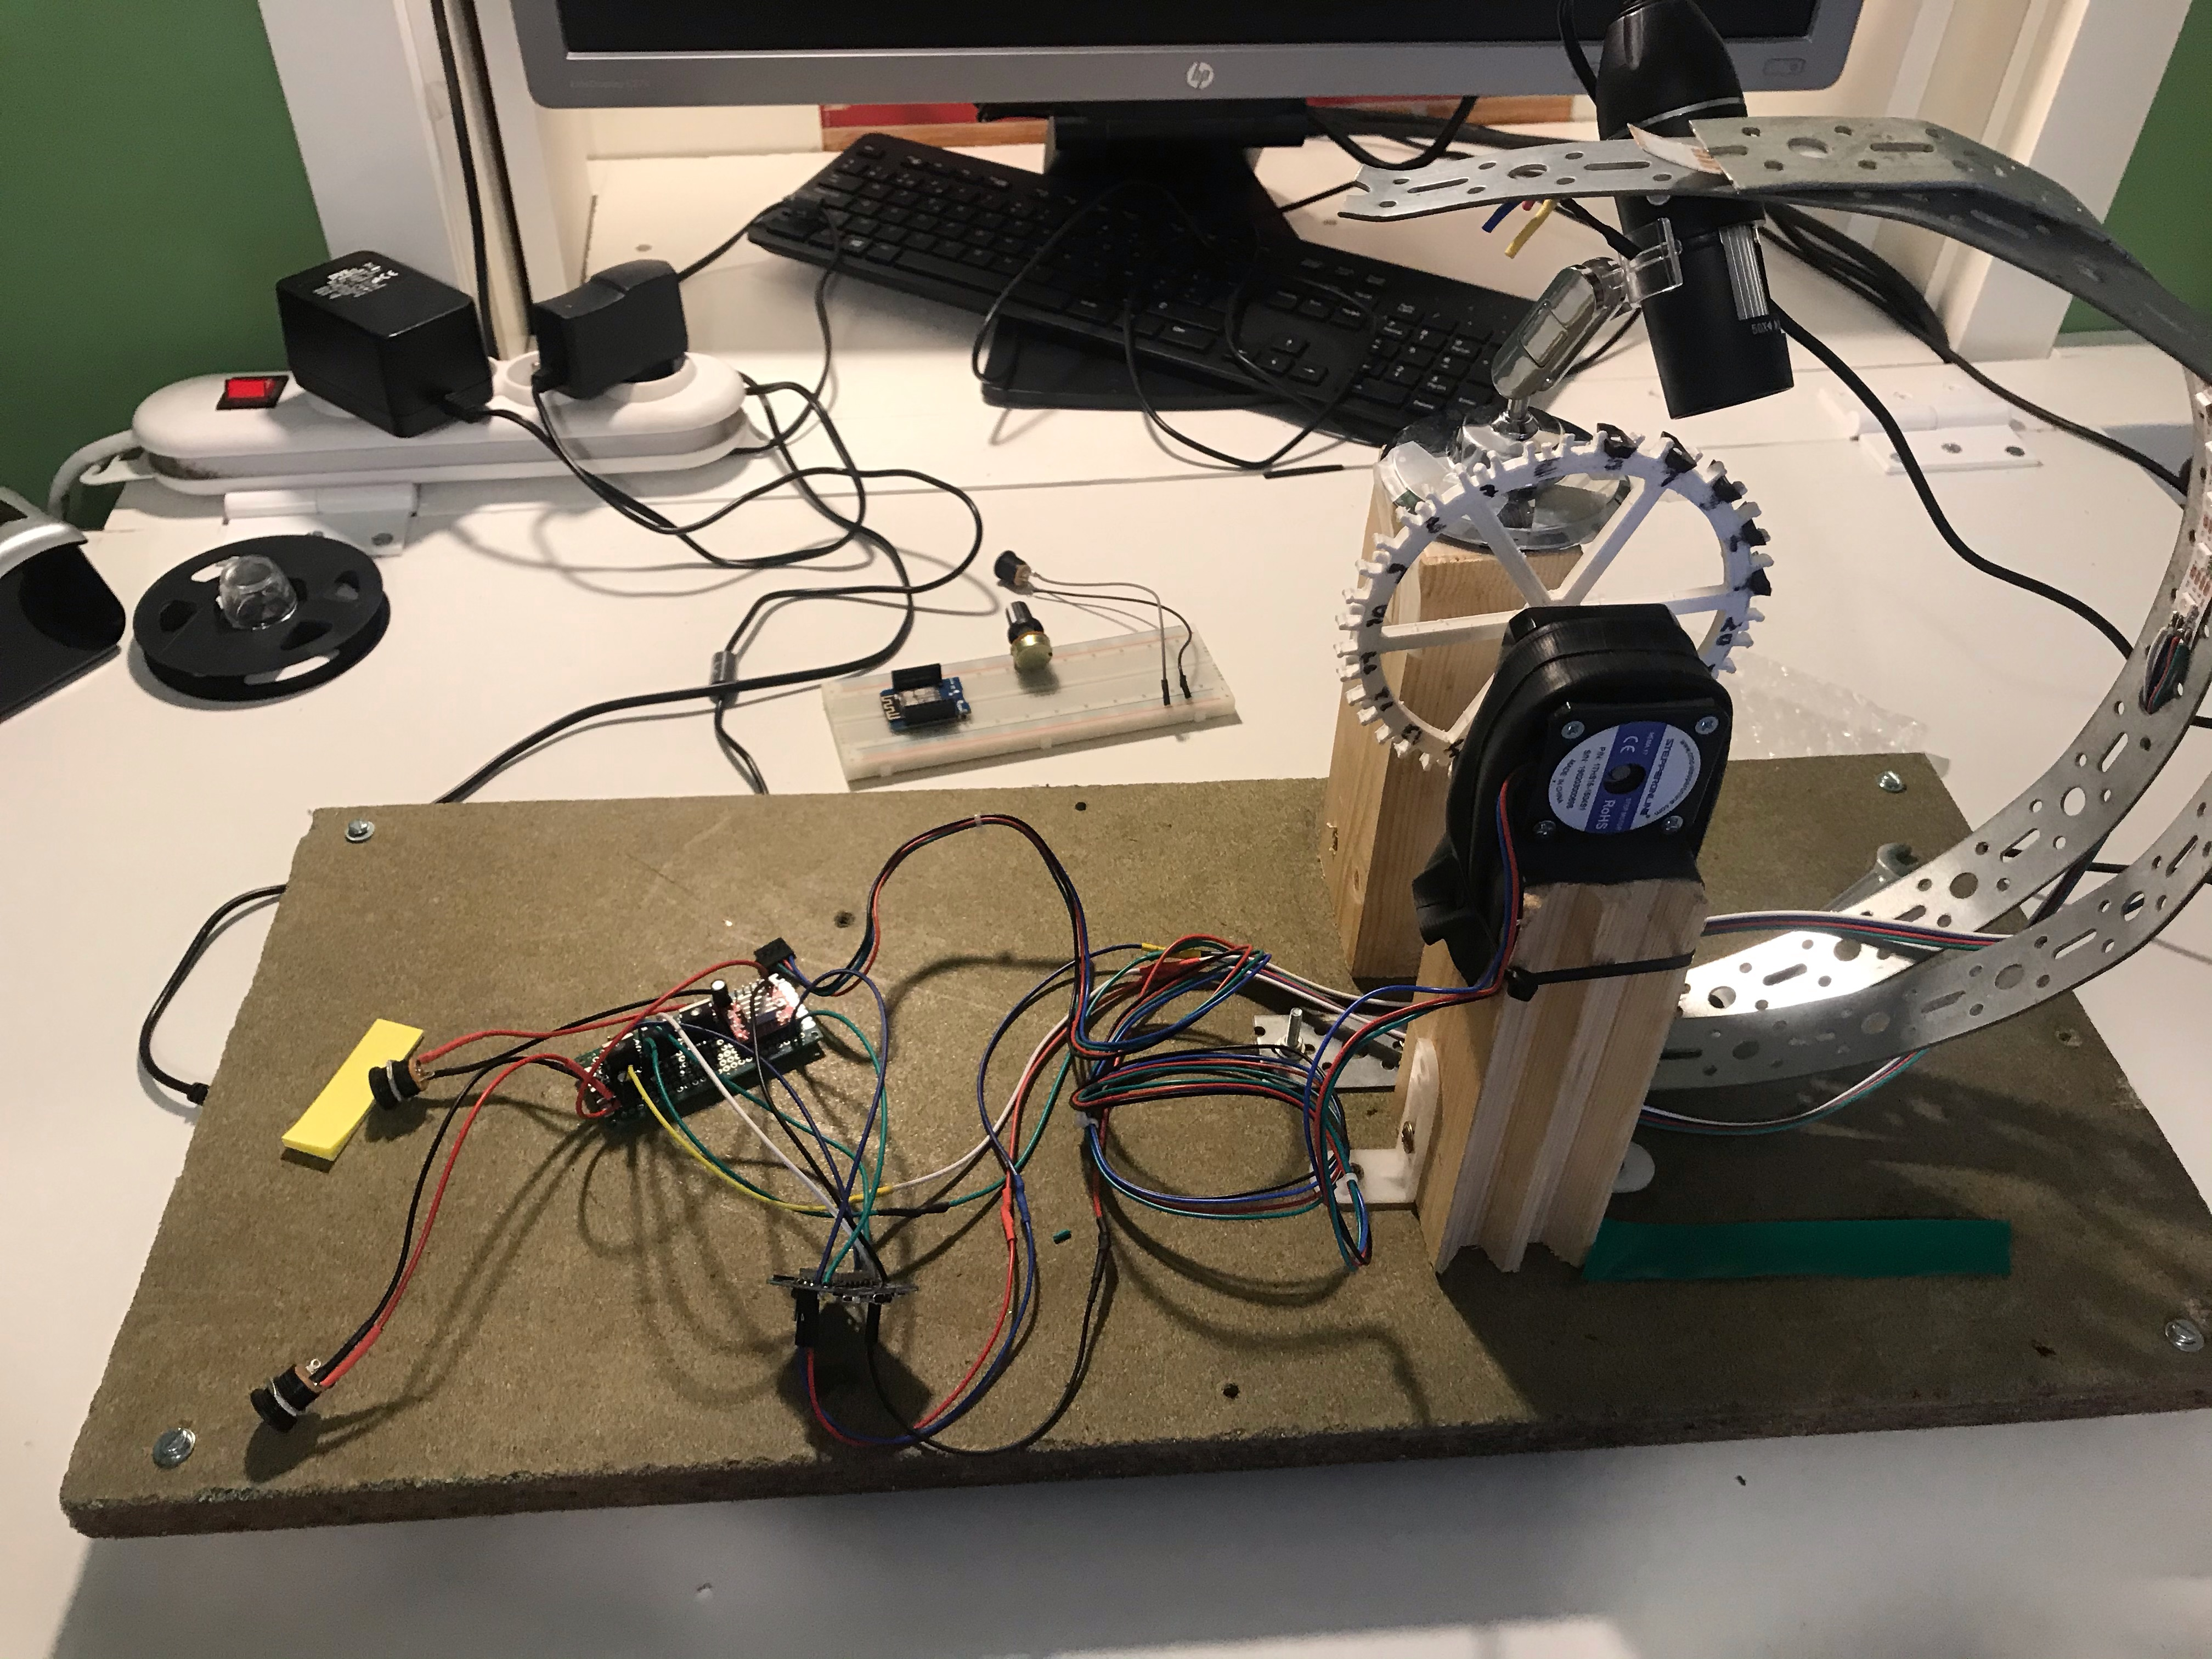
\includegraphics[width=4.166667in, keepaspectratio=true]{./Masterproef_Tool_Wear_Inspection_-_Update_3_DH/rechts_kabels.jpeg}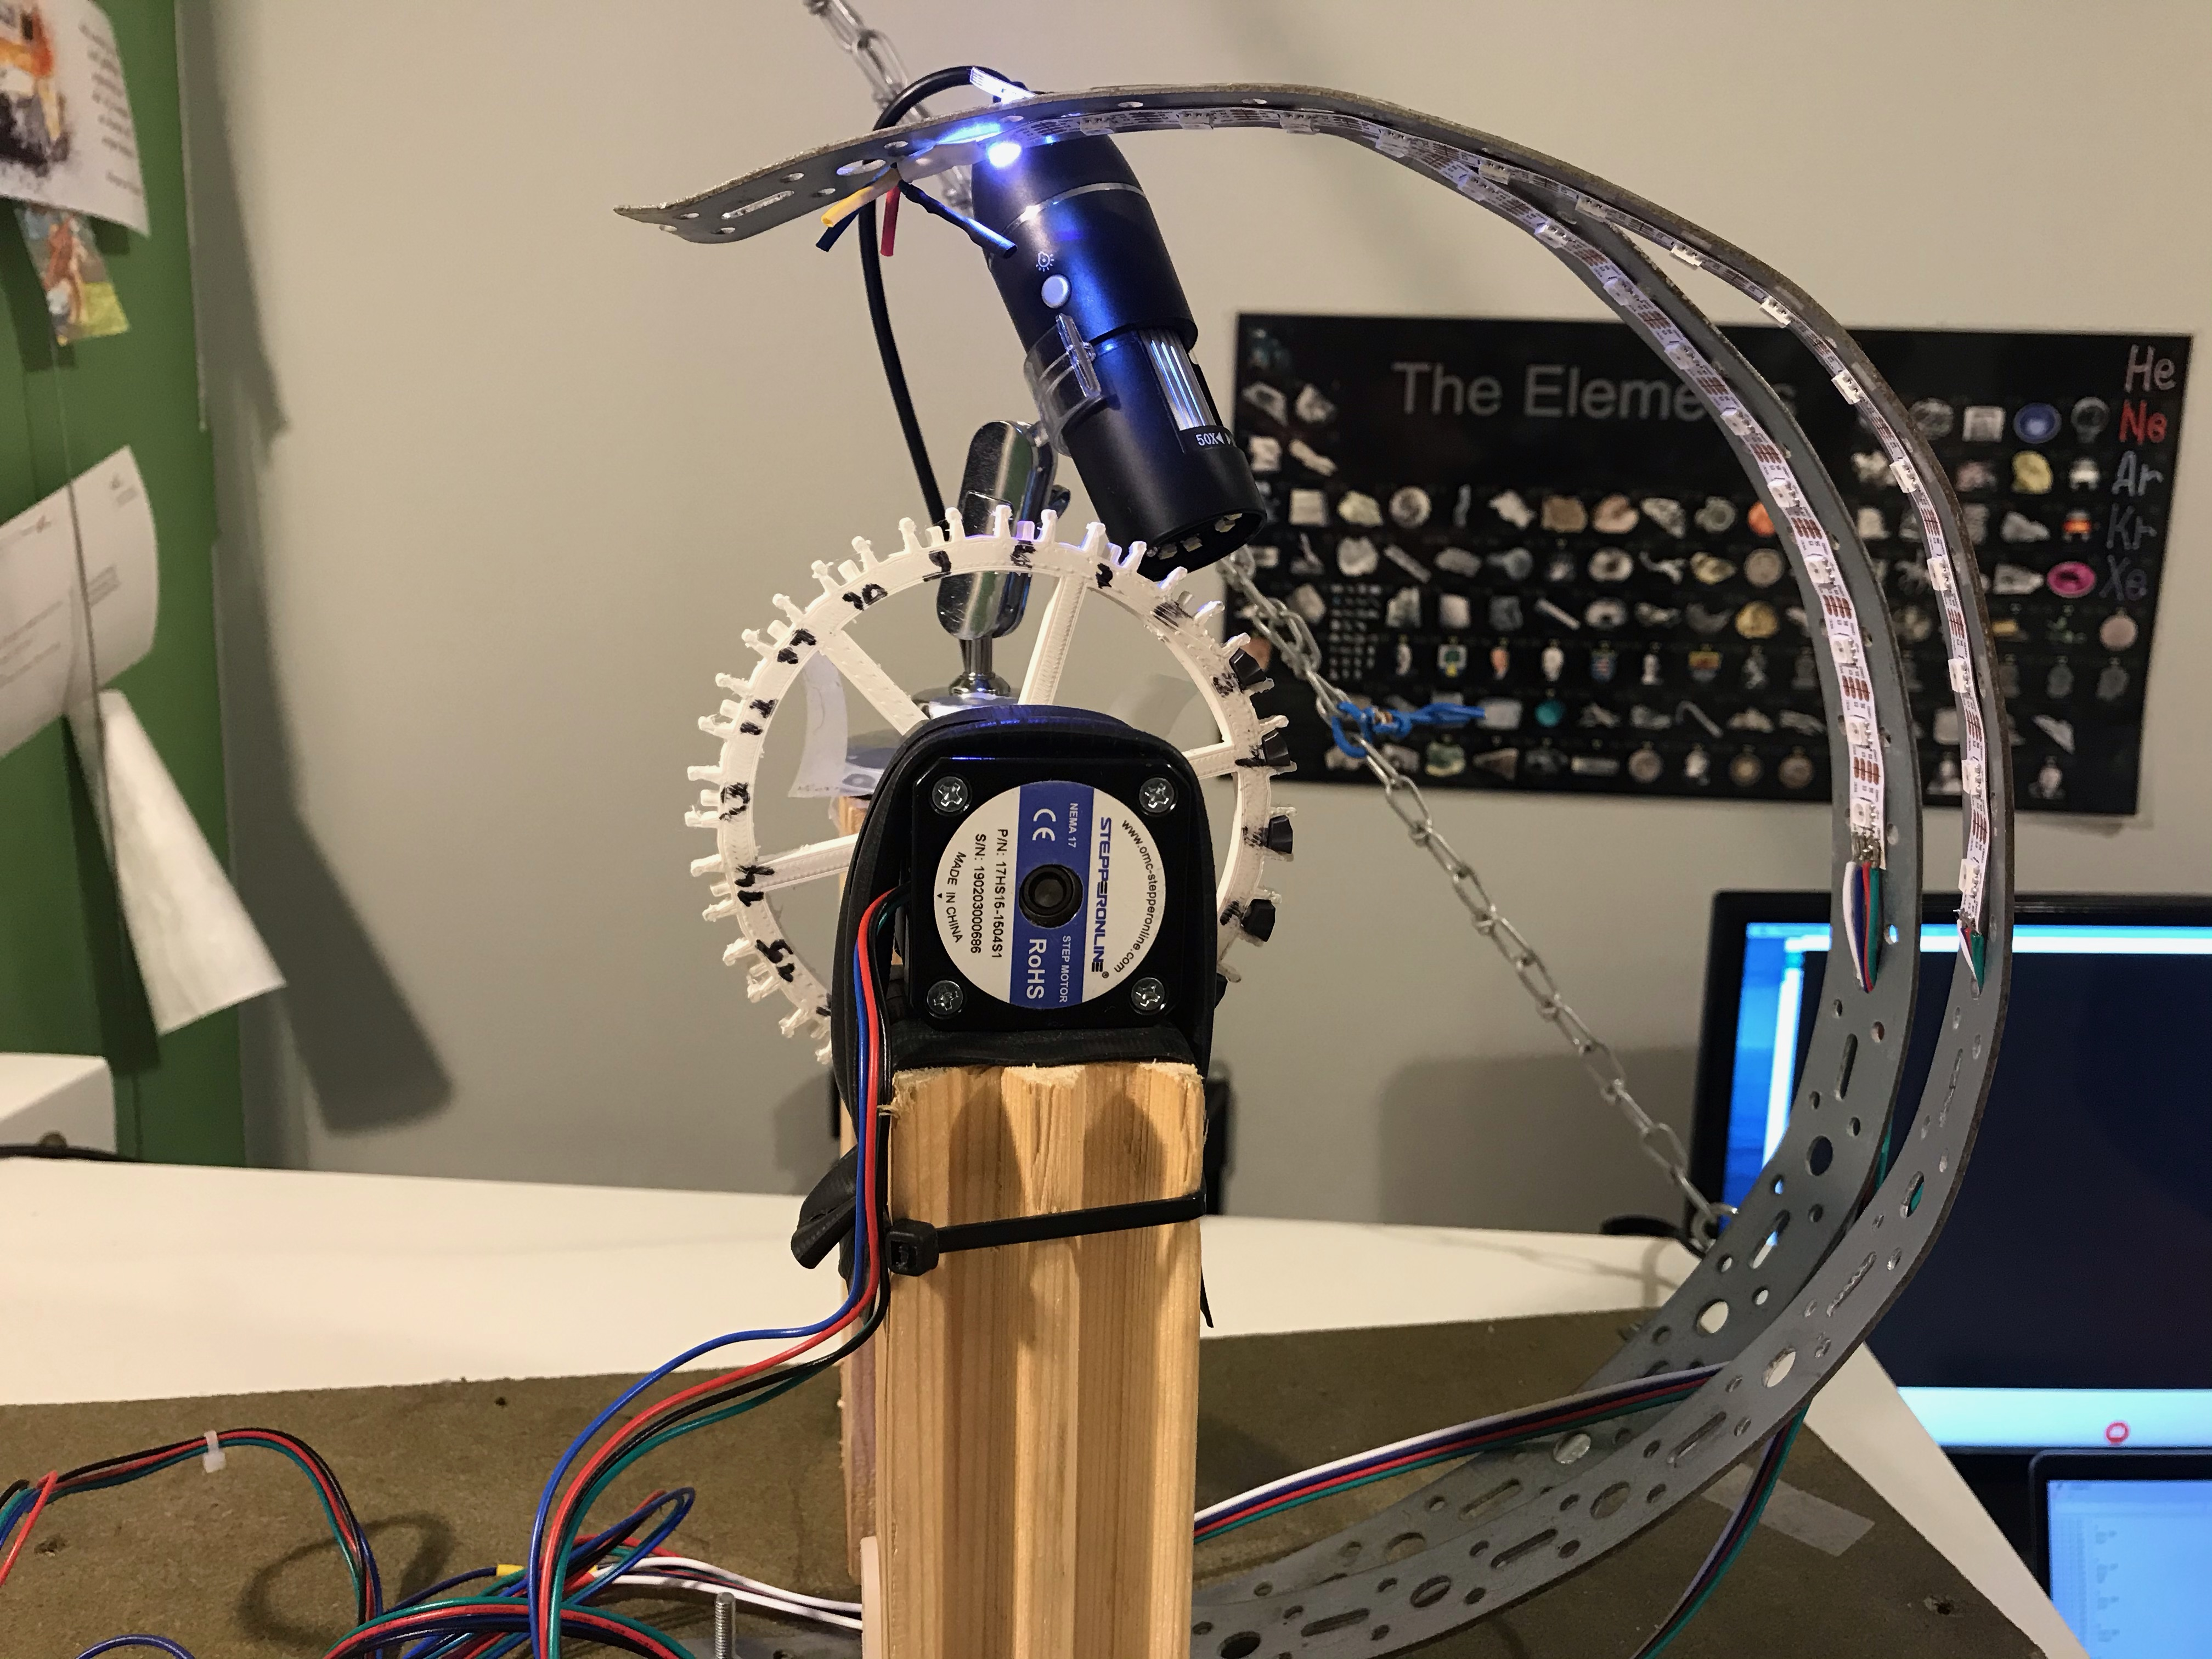
\includegraphics[width=4.166667in, keepaspectratio=true]{./Masterproef_Tool_Wear_Inspection_-_Update_3_DH/rechts.jpeg}

 

Enkele genomen foto’s zitten in bijlage, ik heb hier telkens een foto genomen wanneer twee overeenkomstige leds van de ledstrips branden en al de rest uit om te zien welke leds overeenkomen met welke weerkaatsing in de camera. Op de foto’s is mooi te zien hoe elke led een ander deel van de slijtage belicht.

A picture containing dark, sitting, looking, lit



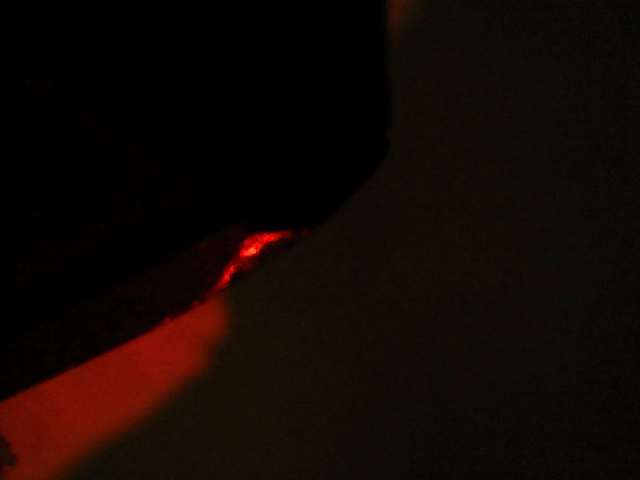
\includegraphics[width=4.166667in, keepaspectratio=true]{./Masterproef_Tool_Wear_Inspection_-_Update_3_DH/p4_l10.png}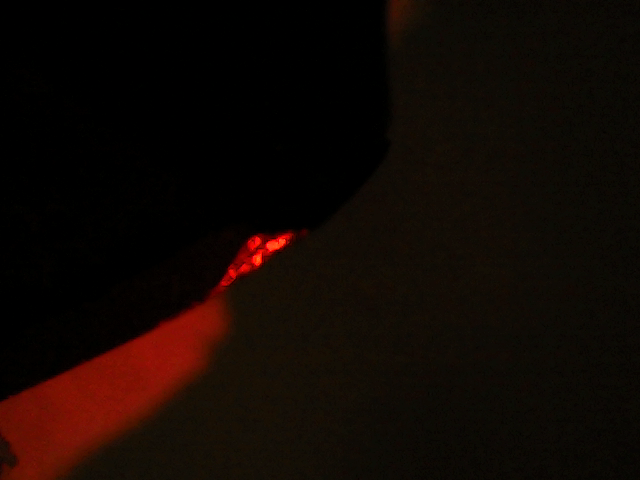
\includegraphics[width=4.166667in, keepaspectratio=true]{./Masterproef_Tool_Wear_Inspection_-_Update_3_DH/p4_l9.png}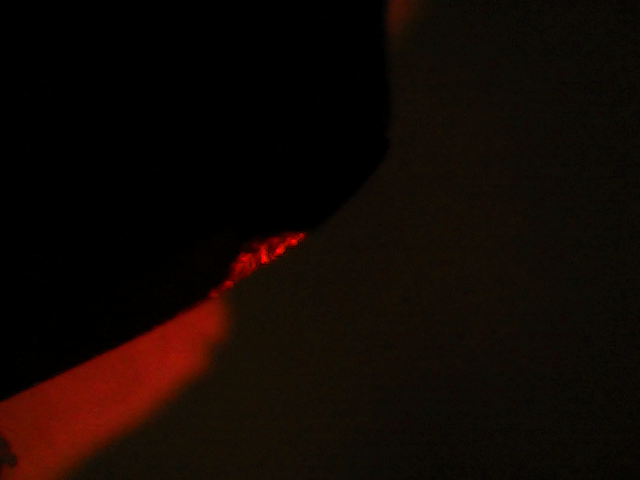
\includegraphics[width=4.166667in, keepaspectratio=true]{./Masterproef_Tool_Wear_Inspection_-_Update_3_DH/p4_l8.png}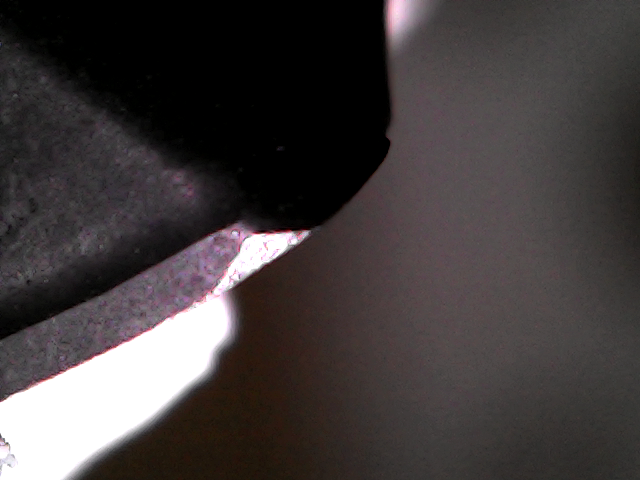
\includegraphics[width=4.166667in, keepaspectratio=true]{./Masterproef_Tool_Wear_Inspection_-_Update_3_DH/p4.png}

 

Hier lijkt de belichting dus wel goed te zitten, maar is er nog licht weerkaatsing van de witte houder waarin de plaatjes zitten. Om dit weg te werken dacht ik er aan om ofwel het rad met zwart filament te printen of het witte rad zwart te verven, ik hoop dat dat de problemen zou oplossen. De andere optie is om er voor te zorgen dat de houder in de schaduw ligt. Dat is echter wat moeilijker gezien de twee ledstrips van een andere hoek belichten.

 

Om de leds en de motor aan te sturen werk ik met een python programma dat via pyserial gegevens doorstuurt naar een Wemos D1 mini, die met de software van arduino werkt, door op zijn poort te schrijven. Dit ging echter heel traag waardoor ik na elk commando 1,5 seconden moest wachten eer ik het volgende commando kon sturen of er iets anders kon gebeuren. Dat zorgde ervoor dat elke foto ongeveer 5 seconden duurde. Dit met 15 verschillende licht settings was niet ideaal dus ik ga de communicatie snelheid nog proberen verhogen en anders een echte arduino gebruiken in de hoop dat dat sneller werkt.

 

De reden dat ik het via deze omslachtige manier doe (via seriele poort naar een arduino) is omdat ik heb geprobeerd om met een raspberry pi alles uit te voeren, aansturing van de leds en de beeld opname, maar dat ging ook vrij traag.

En er is een raspberry pi stuk gegaan door een kortsluiting in het pcb dat ik had gesoldeerd. Om niet nog een raspberry pi kapot te maken ben ik overgeschakeld naar de Wemos D1 mini chips die veel minder duur zijn, wat de gevolgen van een kortsluiting een heel stuk beperkt.

 

Ik heb ook opgezocht of het wolfram carbide waaruit de plaatjes zijn gemaakt bepaalde reflectieve eigenschappen heeft, maar dit was zonder succes. Er waren wel een aantal studies die de licht absorbtie besproken om fouten te herkennen en die lagen vooral in het infrarode spectrum. De echte reflectiviteit zal ik misschien eens proef ondervindelijk moeten uitzoeken.

 

Met vriendelijke groeten,

 

Lars De Pauw



\subsection{Reply}

Hallo Lars,



Dat ziet er al heel goed uit!​ Op de foto's kan je inderdaad duidelijk de slijtage zien. Misschien kunnen we zelf die 4 foto's combineren tot 1 foto, of als je de bijhorende 4 led's gelijktijdig laat branden, krijg je dan het zelfde resultaat? 



De weerkaatsing van de draaischijf kan je inderdaad oplossen met verf of zwart filament. 



Zeker de info bijhouden over lichtabsorbtie in het IR spectrum, dit kan je bij in u literatuurstudie zetten.



Super goed bezig! Dit gaat zeker het resultaat verbeteren, dat je al vertrekt met goede foto's!



Mvg,





\subsection{Mail}

Beste meneer Hulens,

 

Die vier foto’s zelf combineren tot één foto lijkt me de meest stabiele methode gezien de leds niet steeds hetzelfde resultaat geven voor een verschillend plaatje. In bijlage zitten twee foto’s van verschillende plaatjes die met dezelfde leds belicht zijn.



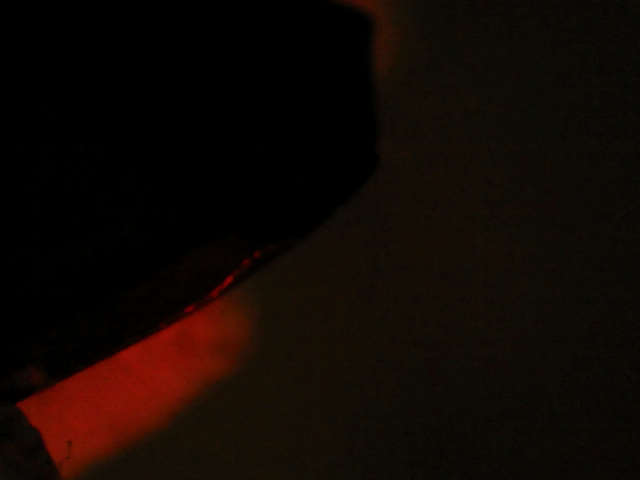
\includegraphics[width=4.166667in, keepaspectratio=true]{./Masterproef_Tool_Wear_Inspection_-_Update_3_DH/p3_l9.png}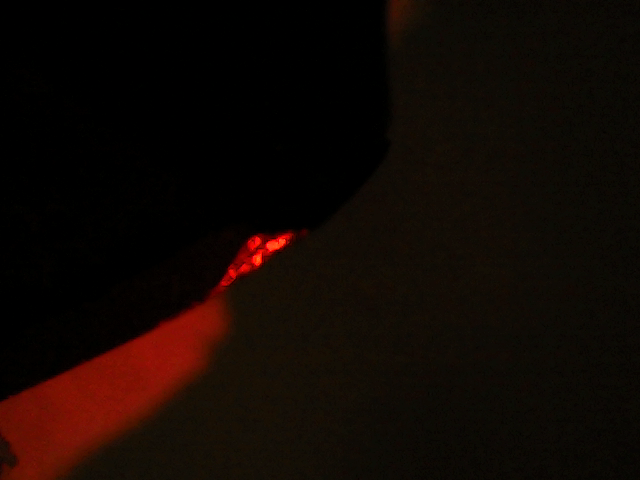
\includegraphics[width=4.166667in, keepaspectratio=true]{./Masterproef_Tool_Wear_Inspection_-_Update_3_DH/p4_l9.png}

 

Dit verschil komt doordat de plaatjes niet allemaal perfect in hun houder zitten en sommige dus een beetje schuin hangen. Dat zou kunnen opgelost worden met een verbetering van de houder en dan kan er in theorie per plaatje gewoon steeds dezelfde leds oplichten. Met de huidige plaatjes die zijn afgesleten met de hand zal dit nog niet tot perfecte resultaten komen gezien de hoek waarin het materiaal is afgesleten niet constant is. -\textgreater{} ik weet nog niet over hoeveel verschil dit gaat, het kan zijn dat dit verschil slecht 5 graden is waardoor het wel zou lukken om 4 leds tegelijk aan te zetten.

De echte plaatjes die met de machine zijn afgesleten zullen normaal gezien wel steeds dezelfde slijtage hoek hebben waardoor dat wel zou werken.

 

Met vriendelijke groeten,

 

Lars De Pauw







\end{document}
